\documentclass[twoside,11pt]{article}
%\documentclass[twoside,10pt]{article}

\usepackage{jmlr2e}
\usepackage{spverbatim}
\usepackage{amsmath}
\usepackage{caption}

\newcommand{\ith}{$i^{th}$ }
\newcommand{\jth}{$j^{th}$ }
\newcommand{\weight}{$w_{ji}$ }
\newcommand{\Rw}{\mathbb{R}^w }
\newcommand{\R}{\mathbb{R}}

\begin{document}

\title{Auto-Encoders for Feature Selection}

\author{\name Andrew Kirby \email andy-kirby@live.com \AND
		\name Kevin Browder \email browderkevin54@gmail.com \AND
		\name Nathan Stouffer \email nathanstouffer1999@gmail.com \AND
		\name Eric Kempf \email erickempf123@gmail.com }

\maketitle

\begin{abstract}
Stacked Auto-Encoders are an unsupervised learning models that can be used for feature selection within datasets. These networks can be trained using Backpropagation and have the ability to place supervised model on top of them for classification and regression tasks. Since each layer (including the predictor network) must be trained, Auto-Encoders take a long time to train.
\end{abstract}

\section{Problem Statement}
	% TODO talk about feature selection stuff
	% TODO mention backprop and ff MLP's in general
	% TODO mention uses of AE (compression and feature selection)
	% TODO include abbreviations (AE)
	Given data sets, the task is to compare the effectiveness and convergence rate for one, two and three layer Auto-Encoders (AE) with a prediction on top of the AE layers. Each version of the Stacked Auto-Encoder (SAE) will be implemented and tested on the following six data sets.
		
	The abalone dataset contains features paired with the age of an abalone (the class). The 28 ages are closely related, potentially making classification difficult.
	The car dataset contains attributes corresponding to 4 possible conditions of a car while the segmentation dataset details 6 distinct subjects of outdoor photographs.
	The rest of the datasets are regression.
	The forest fires set contains the area burned by a forest fire. Most of the values are 0 with a few large values which might give the model trouble.
	The machine dataset predicts the performance of a CPU which has an even distribution across its regression values. Wine quality contains the score of a wine with associated attributes. Several of the attributes are correlated, making regression more difficult \citep{datasets}.
	
	An AE is a type of neural network where the output vector is an approximation of the input vector and the AE tries to learn the function that makes the output as similar as possible to the input. In this case, an AE will be trained using Backpropagation. The power of SAEs lies in their ability to perform feature selection on data sets. These features are then passed into a supervised learning algorithm, an MLP in this case, for classification or regression. This is especially powerful in when features are difficult to obtain or a new application where important features have not yet been identified. 
	
	

\subsection{Hypothesis}
	Fewer AE layers are expected to outperform more AE layers because the datasets used in training are relatively small and there is not enough data to train the deeper SAEs. Additionally, the prediction networks trained will converge faster than the prediction networks trained in Project 3. This is because the features will be linearly independant, which reduces model complexity and training time.
\section{Algorithms}

	Since Backpropagation was explained in a previous project, this paper focuses on explaining an Auto-Encoder. 
	An Auto-Encoder is a feed forward MLP with a single hidden layer. 
	The weights to the hidden layer are often referred to as the encoding layer and the weights to the output layer are called the decoding layer. 
	
	An Auto-Encoder learns a function $f(\vec{v}) \approx \vec{v}$. 
	This is process is now described.
	Take $d,k \in \mathbb{Z}^+$. 
	The encoding layer maps an input vector $\vec{v}_i \in \mathbb{R}^d$ to an encoded vector $\vec{v}_e \in \mathbb{R}^k$.
	The decoding layer then maps $\vec{v}_e$ to $\vec{v}_o \in \mathbb{R}^d$ such that the distance between $\vec{v}_i$ and $\vec{v}_o$ is minimized.
	There is a sense in which the decoding layer is the function inverse of the encoding layer. 
	However, this is not a true inverse relationship since the decoding layer does not produce the exact input given to the encoding layer.
	
	There are two types of Auto-Encoders: undercomplete and overcomplete. 
	An under complete Auto-Encoder is one where $k < d$. This means that the dimensionality of $\vec{v}_e$ is smaller than the dimensionality of the input/output vectors. 
	This forces the encoding layer to reduce the number of features, possibly eliminating linearly dependent features. 
	An undercomplete AE requires tuning to select $k$.
	The other type of AE is overcomplete. This is the case where $k \geq d$.
	Learning this function seems trival since there is an inclusion map $\mathbb{R}^d \mapsto \mathbb{R}^k$.
	However, a sparsity penalty $\lambda \in \mathbb{R}$ is introduced to tend weights in the decoding layer towards 0 (typically $\lambda$ is small).
	That is, at each step in the gradient, each weight is moved towards 0 by a distance of $\lambda$ (subtracting $\lambda$ for positive weights and adding $\lambda$ for negative weights).
	This produces a sparse Auto-Encoder, where some hidden nodes activations are unnecessary because the weights leaving them have a magnitude close to 0.
	At this point, prune out the unnecessary hidden nodes, and it is now be the case that the dimensionality of the hidden layer is less than that of the input/output layer.
	Additionally, the hidden nodes represent the linearly independent features of the data set \citep{sparsity}.
	
	A denoising component can also be added to an Auto-Encoder. To implement this, apply small, random changes to each value in the input vector and then attempt to approximate the original vector by sending the mutated vector through the AE. This will produce a network that denoises data \citep{stacked-ae}.
	
	Auto-Encoders can also be used in a prediction process. Given a trained AE, compute the encoded vector  $\vec{v}_e$ for each $\vec{v}_i$. 
	Then train a feed forward prediction network (such as an MLP) with the encoded vectors. 
	Furthermore, there is no constraint on the number of Auto-Encoders that can iteratively encode the data before a prediction network is trained. 
	The process of iteratively encoding features with Auto-Encoders is called stacking \citep{stacked-ae}.
		
\section{Experiment}

\subsection{Preprocessing Choices}

	First, all the examples in the data set are randomly scrambled and then assigned to sets for ten-fold cross validation. 
	All categorical variables are converted to integers 
	and the preprocessor also generates a similarity matrix for each categorical variable that is used for determining distances between categorical variables. 
	All numerical variables are normalized between 0 and 1. 
	The data sets did not contain any missing variables.

\subsection{Algorithm Choices}
	
	Implementing an Auto-Encoder requires deciding between undercomplete/overcomplete and whether to include denoising.
	For this project, an overcomplete AE was implemented. An overcomplete architecture was chosen so that a sparse AE could be formed that produces linearly independant features in a data set \citep{sparsity}. 
	This reduces the complexity of data sets such as forest fires and wine quality, which have linearly dependant features, making the task of prediction model simpler \citep{datasets}.
	Denoising was not implemented for time's sake.
	
	After the AE architecture has been chosen, there is still the task of choosing the structure of the prediction network.
	For this, a single hidden layer was used. 
	The number of hidden nodes in this layer was two times the dimension of the input vector. This was chosen based on results in a previous project. 
	The number of output nodes was determined whether the data set was classification (with output nodes equal to the number of classes) or regression (with 1 output node).

\subsection{Evaluation Metrics}

	Classification datasets are evaluated with accuracy and mean squared error (MSE). 
	The MSE metric implemented measures the squared error between the predicted and actual class distributions. 
	This is similar in concept to a Brier score but slightly different in computation. Accuracy indicates how well the algorithm individually classifies examples.
	
	To evaluate regression datasets, mean error (ME) and MSE will be used. MSE squares the distance between a real and predicted value, the squares are then averaged over the entire testing set. 
	ME is computed similarly, but will not square the difference. MSE emphasizes the effect of outliers while ME captures whether the learner tends to over or underestimate the values in the test set. 
	MSE and ME are computed using z-scores (the number of standard deviations from the mean) so that comparisons can be made between datasets.

\subsection{Tuning}
	 The parameters to tune are sparsity, denoted $\lambda$, learning rate, denoted $\eta$, and momentum. Due to time constraints there was not time to run tuning. As such, learning rate and momentum were chosen based off of the tuning done in Project 3. Learning rate was chosen to be 0.1 and momentum as 0.25. For sparsity, values are usually close to zero, 0.001 was chosen based on this \citep{sparsity}.
\section{Results}
	For the final run, the parameters chosen for all data sets. The results are shown in Fig. \ref{auto-encoder}. In general, one AE layer performed best on both regression and classification. This realizes the hypothesis that fewer AE layers would perform better. Fewer layers may outperform more layers because of the size of the datasets. All of the datasets are fairly small and there is not enough data in each dataset to train a two layer, much less a three layer, stacked AE. 
	\begin{figure}[h]
		\centering
		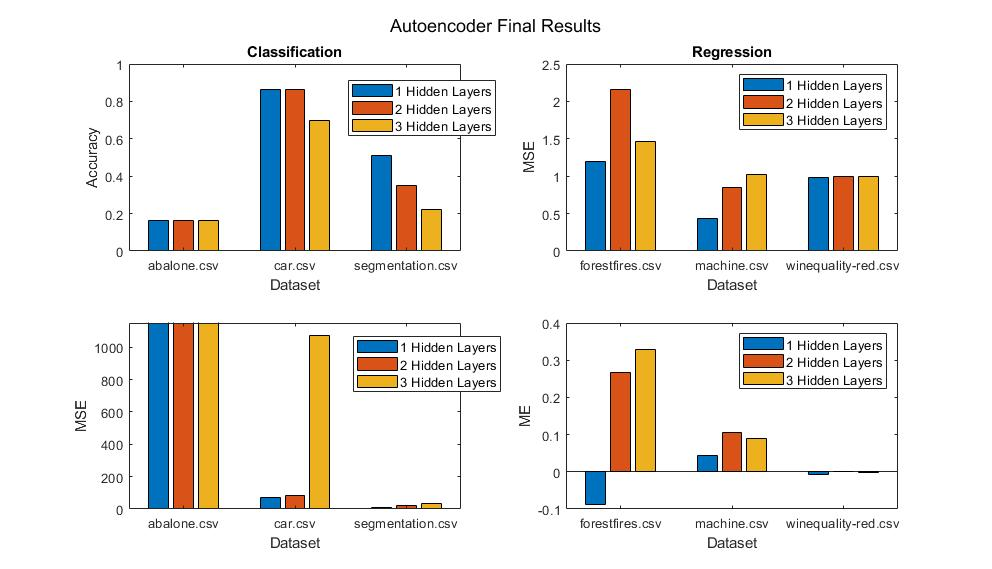
\includegraphics[height=3.4in]{AEresults.jpg}
		\caption{Final Results of 1, 2 and 3 Auto-Encoder layers. Color indicates number of encoding layers.}
		\label{auto-encoder}
	\end{figure}
	The results on car, segmentation and machine perfectly demonstrate the hypothesis. More than one encoding layer significantly decreases performance on all three of these data sets. Abalone and wine quality results were not affected at all by adding AE layers. Abalone performed poorly across the board while wine quality performed quite well. It is likly that the large number of classes in abalone caused even the one layer AE to have insufficient data to train on. Forest fires was the only dataset where three AE layers outperformed two AE layers. This was interesting but the single layer AE still outperformed both the two and three layers AE's on forest fires.
	
\section{Conclusion}
	Stacked Auto-Encoders are unsupervised learning models that excel at feature selection. These networks are trained with Backpropagation. On the assigned datasets, SAEs with one AE layer performed the best. Training of these networks takes a very long time due to the large number of layers that need to be trained before the network is trained as a whole. 
	
	For the assigned datasets a single, AE layer was sufficient and more layers caused a degradation in performance. Larger datasets could benefit from additional AE layers. It all depends on the dataset which brings it back to no free lunch.
\newpage

\bibliography{biblio}

\end{document}
